\chapter{Implementation}
\label{4-practical}

\section{Functionality} 

%% ML: use neni moc vhodne slovo, zkuste preformulovat
%% JP: opraveno na consume (to je, myslim, termin, ktery se v tomto kontextu pouziva)
PyWPS allows to publish and consume geoprocessing services on a
%% ML: zkuste vetu rozdelit (je prilis dlouha, v kratke sekvenci se opakuje 'and')
%% JP: opraveno, snad je to o neco lepsi
server. Every process that is to be implemented by PyWPS must be
constructed as a Python class and contain a list of inputs and outputs.
Also, there must be a handler method with two parameters - request and
response. \cite{pywpsprocess} Details on the procedure of creating new
processes can be found in PyWPS documentation.

%% ML: For sending (?)
%% JP: tady bych asi radeji nechal puvodni formulaci, prijde mi prirozenejsi a vyznamove prakticky stejna
%% ML: running at a server?
%% JP: upraveno
To send a request to PyWPS, an instance of PyWPS must be running at a server.
%% ML: If it is bych asi uplne vynechal
%% JP: smazano
The request is handled and a response is generated and returned
%% ML: file -> document
%% JP: upraveno
%% ML: and -> which ?
%% JP: upraveno {and -> that)
to the client. The response has a form of an \zk{XML} document that
contains different elements depending on the type of the request.

When an Execute request is called, a new, temporary folder is created
%% ML: moved -> copied (nejsou odstranena ze zdroje)
%% JP: upraveno
in location specified in configuration file and input data is copied
here. While the process is being executed, temporary files may be
generated in this folder. For every process, it must be specified what
the final output is. Once the execution is finished, the output is
copied to a location that is accessible via the web. The temporary
folder, containing input and output data and all the intermediate data
that arose during the execution, is then deleted.

\subsection{Output Data Management}

\subsubsection{Current Options} 

The simplest option of delivering output data is to embed it in the
\zk{XML} response document. Either as plain text, \zk{GML} or, in case
%% ML: encoding scheme
%% JP: upraveno
of an image, encoding scheme. This is typically used when the output is
%% ML: where - for PyWPS
%% JP: upraveno, ale myslel jsem, ze to vyplyva z kontextu, cela kapitola se zabyva PyWPS
relatively small. For PyWPS, it is also the default option.

%% ML: u obrazku, ktere jste vytvarel uvedte take zdroj (source: author)
%% JP: dopsano
\begin{figure}[H] \centering
  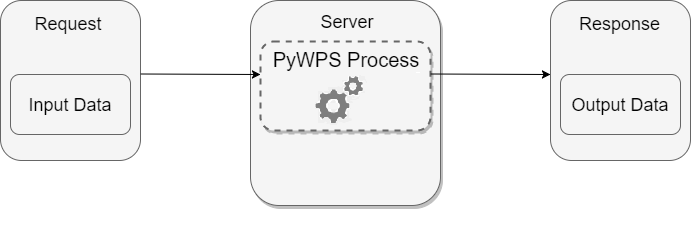
\includegraphics[width=350pt]{./pictures/optionone.png}
  %% ML: zkuste popisek rozsirit, konkretizovat (data odkud kam)
  %% JP: dopsano
      \caption[Delivering output data directly to the client]{Delivering output data directly to the client (source:{author})}
      \label{fig:optionone}
  \end{figure}
  

  If, on the contrary, the output data is large and complex, there is
  another option. The client is only given a reference, a \zk{URL}
  link, from which the data can be downloaded. PyWPS saves the file in
  a folder specified in configuration passed by the service (or in a
  default location). The \zk{URL} is embedded in the \zk{XML}
  response. \cite{pywpsurl}

  %% ML: u obrazku, ktere jste vytvarel uvedte take zdroj (source: author)
  %% JP: dopsano

\begin{figure}[H] \centering
  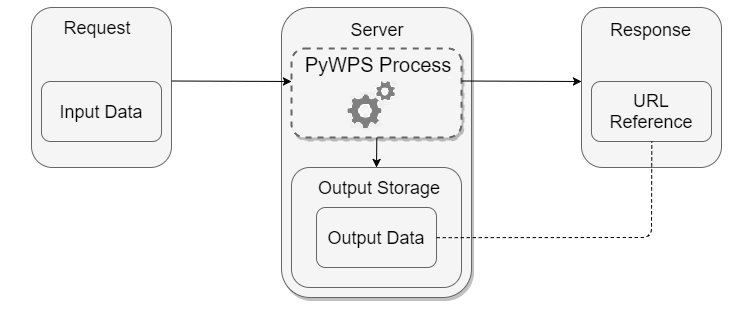
\includegraphics[width=370pt]{./pictures/optiontwo.png}
  %% ML: opet mirne konkretizujte
  %% JP: dopsano
      \caption[Delivering output data via \zk{URL} reference]{Delivering output data via \zk{URL} reference (source:{author})}
      \label{fig:optiontwo}
  \end{figure}

  It is up to the consumer of the process to decide which option to
  choose. For the latter option, the \texttt{"@asReference"} value
  must be set to \texttt{"True"} in the request. \cite{asref} By
  default, it is set to \texttt{"False"}.


\subsubsection{Proposed Extension} 

%% ML: veta nedava moc smysl, prepiste
%% JP: mne smysl dava, konzultoval jsem to s rodilym mluvcim a jemu take. 
%% JP: mate vyhrady z pohledu stylistickeho, nebo vyznamoveho?
%% JP: muzu napsat neco jednoducheho jako "In this thesis, a third
%% JP: option was developed that stores data in a PostGIS database.",
%% JP: ale za sebe nevidim duvod
The aim of this thesis was to develop another variant to add to the
existing two that stores output data in a PostGIS database.

From the point of view of the consumer of a process, it is similar to
the previous option. After the final output has been produced,
connection to the database is established and the output data is
copied there. When the \zk{XML} response is delivered to the client,
%% ML: to neni uplne presne, bude potrebovat pristupove udaje (host
%% name, username, password), viz poznamka nize - jde o jakysi
%% mezikrok 
%% JP: upraveno
it contains a reference that points to the location of the data 
within the database. The reference is composed of the name of the database, schema and table. To access the data itself, database login credentials are neccessary.

The current state is not definitive. In the final state, the client will receive a URL link that references to a \zk{WFS} service. The \zk{WFS} service itself will access the output data stored in a database and serve them to the client. 

%% ML: doplnte, ze jde o mezikrok (poskytnout referenci na databazi)
%% reseni by se melo doplnit o podporu mapoveho serveru tak, aby
%% klient dostal URL WFS sluzby (ta bude data cist z DB). Pote bude
%% reseni ciste (z pohledu OGC standardu)
%% JP: doplneno


\begin{figure}[H] \centering
  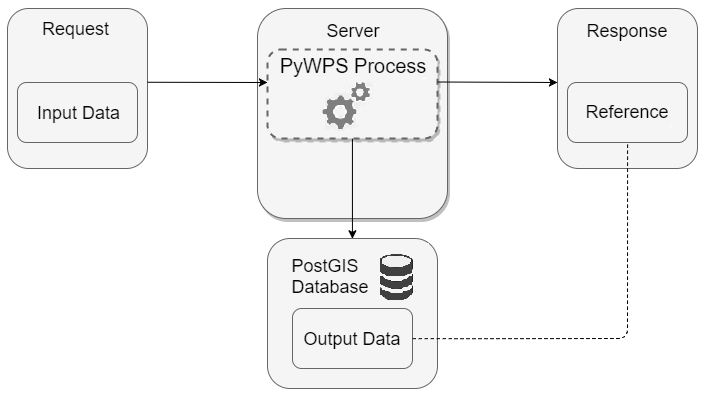
\includegraphics[width=350pt]{./pictures/newoption.png}
    %% ML: opet mirne konkretizujte + zdroj 
    %% JP: doplneno
      \caption[Storing output data in a remote database]{Storing output data in a remote database (source:{author})}
      \label{fig:newoption}
  \end{figure}


To use this functionality as a consumer of a process, it must be implemented in the process by its author. For details on implementation when creating a process, please refer to appendix \ref{appendix}.


\section{Development} 

\subsection{PgStorage class development} 

A new class, \texttt{PgStorage}, has been developed that implements
%% ML: konkretne pro PostGIS (zde by se hodil odkaz do nove kapitoly v
%% technologiich)
%% JP: upraveno, dopsana reference na kapitolu v teorii, kde je PostGIS mezi prost. databazemi
PostGIS storage support. Details on PostGIS can be found in section
 \ref{postgis}. \texttt{PgStorage} is a derived class, inheriting from
\texttt{StorageAbstract} class that is part of PyWPS \zk{API}.
%% part of PyWPS API
%% JP: upraveno

%% ML: uvadejte pywps/iout (zpetna lomitka je Windows notace, ktera
%% zde neni podstatna)
%% JP: upraveno
%% ML: misto adresarich mluvte radeji o Python modulech
%% JP: upraveno
PgStorage is stored within \texttt{storage.py} in the ./
pywps/inout module. It consists of several methods that
are described below.

\subsubsection{\textunderscore \textunderscore init\textunderscore \textunderscore } 
A constructor, i.e. it gets called automatically when an instance of
the \texttt{PgStorage} class is created.

In this method, the \texttt{get\textunderscore config\textunderscore
  value} function is used that is defined within the PyWPS API. It
accesses the configuration file and retrieves required elements. What
elements are retrieved is specified by the function's two parameters,
section and option.

%% ML: ten popis je mozna prilis detaily, polopatisticky a spatne se
%% cte, muzete zkusit zkratit / zprehlednit
%% JP: trochu preformulovano
Correct section (\texttt{db}) is specified and saved to a
variable. The name of the database is extracted from the
configuration file and saved to a variable.

Another variable is defined that serves as a connection string for
connecting to a database. Requisite elements (user name, password and
host server) are retrieved from the configuration file. Finally, an
instance of the \texttt{\textunderscore create\textunderscore schema}
method is created and saved to a variable. See an example of a \texttt{db}
section in section \ref{cfgchanges}.


\subsubsection{\textunderscore create\textunderscore schema} 

%% ML: Opet, ten popis je prilis detailni, nevede to k citelnosti
%% textu, neni to zasadni vytka, klidne nechte, mebo mirne upravte
%% JP: zkraceno
First defines a variable \texttt{schema\textunderscore name} as a
random string of specified length that consists of letters and
digits. This is done using Python libraries \texttt{random} and
\texttt{string}.
 
%In the future, schema_name should be created in another way so it is related to the process

\texttt{Psycopg2} library is used to connect to database
specified by the target variable. A try-except clause is included to raise
an exception if the connection cannot not be established.

Then, when a cursor has been created, an \zk{SQL} query is executed
that generates a new schema if it doesn't exist already. Changes in database are
commited so they persist after connection is aborted, cursor and
connection are closed and the \texttt{schema\textunderscore name}
variable is returned.

\subsubsection{\textunderscore store\textunderscore output}

%% ML: na tomto miste bych spise nez o knihovne OGR mluvil o GDAL
%% (muzete pridat link do technologii, aby byl text lepe provazan)
%% JP: upraveno, pridan link
As its name suggests, it handles writing output data to the
database. It benefits from an extensive use of GDAL library. More
information about GDAL can be found in section \ref{gdal}. It has
two input parameters, the name of the file that is to be stored in a
database, and a process identifier.

Thanks to GDAL, the process is fairly simple and straight-forward. The
output file is opened using the file name input parameter and
connection to the database is established. Then, data is copied from
the output file to the database using the OGR \texttt{CopyLayer}
function.

Each of the three above mentioned operations is followed by a simple
condition that checks if the variable storing output of the operation
is not None. If it is, it raises an exception with a corresponding
message.

This method returns the identifier.


\subsubsection{store} 

The store method is defined in the \texttt{StorageAbstract} parent
%% ML: muzete uvest, ze output je v tomto pripade instance tridy ComplexOutput 
%% JP: doplníno
class. Just as in the parent class, it has \texttt{output} as an input
argument. In this case, output is an instance of the ComplexOutput class.

It initializies the \texttt{\textunderscore store\textunderscore
  output} method and passes it name and identifier of the output file.

Then, a string is created that specifies the location of the data and
saved as a variable. It consists of a name of the database, schema and
identifier. This string is then given to the client as an output in
the \zk{XML} response of the process.

There are three parameters returned by the method - the corresponding
value of a DB variable defined within the \texttt{STORE\textunderscore
  %% ML: nazev vystupniho souboru neni v soucasnosti nijak pouzit 
  %% JP: nerozumim. co mam zmenit? metoda prece nazev opravdu vraci, at
  %% uz se pak pouziva, nebo ne.  
  TYPE} class, name of the output file and the variable describing the
%% ML: zduraznete ze jde o DB
%% JP: tady take nerozumim
location of the data. These must be returned as they are required by
the \texttt{get\textunderscore url} method (defined within the
%% ML: presne, viz poznamka vyse
\texttt{ComplexOutput} class).


\subsection{PyWPS source code changes} 

All changes that have been done within the PyWPS source code can be
%% ML: zde uvedte odkaz do prilohy 
examined in a \texttt{diff} folder that is appended to this thesis.
%% ML: diff bude pravdepodobne pouze jeden, vetu muzete vynechat
%% JP: smazano (predpokladal jsem, ze se pro kazdy modul vytvori sam. diff soubor)

%% ML: tyto zmeny nejsou aktualni!!! v tride Process jiz v soucasnosti
%% zadne zmeny nejsou (pokud se nepletu), text je potreba upravit na
%% zaklade nasi posledni schuzky
%% ML: v kodu jsem odstranil pozustatek zmen (583b5ea), nyni by ve
%% tride Process jiz zadne zmeny byt nemely
%% JP: vychazel jsem z toho jak trida vypadala, kdyz jsem kapitolu psal. ted tedy celou kapitolu mazu

%% ML: Output.py neni trida ale Python modul
%% JP: opraveno
\subsubsection{Outputs.py module}

This module includes three classes that define how outputs are handled and delivered to the client. Each class deals with one type of output data - Literal, Complex and BoundingBox.
%% ML: muzete uvest jake tridy tento modul poskytuje (ani ne jejich
%% vycet), ale logicky ramec funkcionalit techto trid (vystupni typy
%% parametru)
%% JP: doplneno
Since there is another option being added of storing output data that
returns a reference to the client, \texttt{\textunderscore
  %% ML: uvadite metodu, jake tridy, 
  %% JP: doplneno
  execute\textunderscore xml\textunderscore reference} method in \texttt{ComplexOutput} class had to
be adjusted.

Whether the output data is stored as a file or in a database depends
on value of the \texttt{store\textunderscore type} option in
configuration file. \texttt{store\textunderscore type} is a new
variable within the configuration file that was declared for
this purpose. For details on changes in the configuration file,
refer to section \ref{cfgchanges}. The code block that has been added here
%% ML: toto je nova konfiguracni promenna (to byste mel zminit)
%% JP: pridano
first retrieves the value using \texttt{get\textunderscore
  config\textunderscore value}. If it is equal to \texttt{"db"},
\texttt{PgStorage} is chosen to handle output data. In any other case
(the value is different or the option is missing),
\texttt{FileStorage} is used.

%% ML: opet jde o modul, doplnte jake tridy tento modul obsahuje
%% JP: opraveno, doplneno
\subsubsection{Storage.py module}

\texttt{PgStorage} class has been added that implements the
database storage functionality. For more details on this class,
refer to the section 4.2.1. 

\texttt{FileStorage} is another class defined in this module that inherits 
from \linebreak the \texttt{StorageAbstract} class. As described above, 
it is either this class or  \texttt{PgStorage} that gets called 
when a reference is to be returned within the response document. 
As its name indicates, it saves outputs as files.

There is another class called \texttt{get\_free\_space} within
this module. Its name, too, is self-explanatory - it returns
folder or drive free space.

%% ML: nasledujici dva odstavce jsou duplicitni
%% JP: duplikat odstranen
Also, second option has been added to the class
\texttt{STORE\textunderscore TYPE}.  So, apart from a \texttt{PATH}
variable that implies storing output data as a file, there is also a
\texttt{DB} variable that is used when saving data in a database.

%% ML: testing?
%% JP: myslel jsem to jako odkaz na nazev skriptu (test), ale je to jedno. upraveno
\subsection{Testing} 

A script has been developed to test whether the process of storing
outputs in a database functions correctly.

For the purpose of this test, three simple processes have been
written. One of them only returns a string, while the other two,
%% ML: text preteka, opravte
(\texttt{process\_one\_output} and \linebreak
\texttt{process\textunderscore two\textunderscore outputs}), produce
one and two complex outputs, respectively.

%% ML: zde zminte, ze jde o processy do znacne miry inspirovane
%% procesem z pywps flask demo!
%% JP: mam tam vetu: "They are based on sample processes available for the PyWPS
%% demo service." mam to jeste nejak zduraznovat, nebo to takto staci?
Both \texttt{process\textunderscore one\textunderscore output} and
\texttt{process\textunderscore two\textunderscore outputs} generate
buffers around input features, the latter also calculates centroids
thereof. They are based on sample processes available for the PyWPS
demo service. There is also a \zk{GML} file provided with the demo
service that was used as an input file for this test.

To sucessfully run the test, instance of PyWPS must be running. When
run, the test executes each of the processes and analyzes the
corresponding \zk{XML} response using the ElementTree \zk{XML}
parser. For every process, it returns an identifier of the process
extracted from the \zk{XML} document.

For the two processes that yield complex outputs the test establishes
connection to the database and counts features in the corresponding
table. Then it compares this value to the number of features in the
input file. If these two values differ, it raises an exception.

Similarly, it checks whether the geometry type of the layer in
database is equal to a predefined value (point for centroids, polygon
for buffer). If not, it raises an exception with a corresponding
warning.

When no exception is raised, it indicates that all processes have been
run and all complex outputs have been stored in a database.

%% ML: OGR -> GDAL
%% JP: upraveno
GDAL library is used for creating database connection, counting
features and getting geometry type. Database login credentials are
retrieved from a configuration file using \texttt{get\textunderscore
  config\textunderscore value}. To ensure correct configuration file
is read, another PyWPS built-in function, \texttt{load\textunderscore
  configuration}, is used.
For information on how to download all required data and run the test,
refer to appendix \ref{testing}.

%% ML: pokud bude v priloze ukazka spusteni, tak zde uvedte link
%% JP: doplnil jsem

%% ML: podobne by mela byt v priloze ukazka konfigurace (v textu
%% konfiguraci na vice mistech zminujete, doplnte linky do prilohy)
%% JP: v priloze 2 mam ukazku sekce db + store_type=db; staci to tak,
%% nebo jste mel na mysli cely konfiguracni soubor?
